\documentclass[dvipsnames]{beamer}
% \mode<presentation>{}
\usepackage[utf8]{inputenc}
\usepackage{amsmath, amssymb, amsfonts, amsthm, mathtools, mathrsfs}
\setbeamertemplate{theorems}[numbered]
\title{Coordinate Hit-and-run}
\author{Amit Rajaraman}
\date{\today}
% \institute{IIT Bombay}
\usetheme{Madrid}
\usepackage{parskip}
\usepackage{tcolorbox}
% \usepackage{tikz-cd}
% \usepackage{commands}
\usepackage{graphicx}
% \usepackage{soul}

% \usepackage{tikz}
% \usetikzlibrary{topaths,calc}
\usepackage{caption}
\usepackage{subcaption}
\usepackage{cancel}
\usepackage{commath}
\usepackage{sansmathaccent}
\pdfmapfile{+sansmathaccent.map}
\usepackage[absolute,overlay]{textpos}
\usepackage{framed,fancybox}
\usepackage{tcolorbox}
\definecolor{foo}{rgb}{0.2,0.2,0.7}

\newcommand\colorfbox[3]{%
 {\color{#1}\fbox{\parbox{\dimexpr\linewidth-2\fboxsep-2\fboxrule\relax}{\color{#2}#3}}}%
}


% \newenvironment{cframed}
%   {\def\FrameCommand{\fboxsep=\FrameSep\fcolorbox{blue}{white}}%
%     \MakeFramed {\advance\hsize-\width \FrameRestore}}
%   {\endMakeFramed}

% \renewcommand\fbox[1]{\Ovalbox{#1}}
\newcommand\MyText[1]{
  \begin{textblock*}{5cm}(.7\textwidth,0.7cm)
    \colorfbox{foo}{black}{#1}\phantom{.}
    % \begin{cframed}
    % 	#1
    % \end{cframed}
  \end{textblock*}
}

\setbeamerfont{bibliography entry author}{size=\small}
\setbeamerfont{bibliography entry title}{size=\small}
\setbeamerfont{bibliography entry location}{size=\small}
\setbeamerfont{bibliography entry note}{size=\small}
\setbeamerfont{bibliography item}{size=\small}


% \tikzset{
%     invisible/.style={opacity=0},
%     visible on/.style={alt={#1{}{invisible}}},
%     alt/.code args={<#1>#2#3}{%
%       \alt<#1>{\pgfkeysalso{#2}}{\pgfkeysalso{#3}}%
%   }
% }

\makeatletter
\newenvironment<>{proofs}[1][\proofname]{%
	\par
	\def\insertproofname{#1\@addpunct{.}}%
	\usebeamertemplate{proof begin}#2}
  {\usebeamertemplate{proof end}}
\makeatother

\newcommand{\R}{\mathbb{R}}
\newcommand{\Rp}{\mathbb{R}^+}
\newcommand{\Rn}{\mathbb{R}^n}
\newcommand{\N}{\mathbb{N}}
\newcommand{\Z}{\mathbb{Z}}
\newcommand{\Q}{\mathbb{Q}}
\newcommand{\vol}{\operatorname{vol}}
\newcommand{\diam}{\operatorname{diam}}
\newcommand{\rad}{\operatorname{rad}}
% \newcommand{\norm}[1]{\left\lVert#1\right\rVert}
\newcommand{\grad}{\nabla}
\newcommand{\opnorm}[1]{\norm{#1}_{\text{op}}}
\newcommand{\indic}{\mathbbm{1}}
\renewcommand{\d}[1]{\ensuremath{\operatorname{d}\!{#1}}}
\newcommand{\expec}{\textbf{E}}
\newcommand{\Var}{\operatorname{\textbf{Var}}}
\newcommand{\conv}{\operatorname{Conv}}
\newcommand{\vr}{\operatorname{vr}}
\newcommand{\avg}{\operatorname{avg}}
\newcommand{\med}{\operatorname{med}}
\newcommand{\uvol}{\underline{\vol}}
\newcommand{\ovol}{\overline{\vol}}
\newcommand{\Span}{\operatorname{span}}
\newcommand{\evol}{\widetilde{\vol}}
\newcommand{\Int}{\operatorname{Int}}
\newcommand{\Tr}{\operatorname{Tr}}


% \setbeamercolor{footline}{fg=brown}
% \setbeamerfont{footline}{series=\bfseries}
% \addtobeamertemplate{navigation symbols}{}{%
%     \usebeamerfont{footline}%
%     \usebeamercolor[fg]{footline}%
%     \hspace{1em}%
%     [\insertframenumber/\inserttotalframenumber]
% }

\theoremstyle{definition}
\newtheorem{thm}{Theorem}
\newtheorem{defn}[thm]{Definition}
\newtheorem{prop}[thm]{Proposition}
\newtheorem{cor}[thm]{Corollary}
\newtheorem{caution}[thm]{Caution}
\newtheorem{ques}{Question}
\newtheorem*{ques*}{Question}
\newtheorem*{alg}{Algorithm}
\newtheorem*{fac}{Fact}
\newtheorem*{ex}{Example}
\newtheorem{lem}[thm]{Lemma}


% \DeclareMathOperator{\len}{len}
% \newcommand{\md}[1]{\left\lvert #1 \right\rvert}

\AtBeginSection[]
{
  \begin{frame}
	\frametitle{Table of Contents}
	\tableofcontents[currentsection]
  \end{frame}
}

\begin{document}
\begin{frame}
	\titlepage
\end{frame}

\begin{frame}
	\frametitle{Table of Contents}
	\tableofcontents
\end{frame}

\section{Introduction}
\begin{frame}{The problem}
	Uniformly sampling points from a high-dimensional convex body is a basic problem that relates to problems such as volume computation of convex bodies in high dimensions. \pause \\
	\begin{defn}
		A compact convex body $K \subseteq \Rn$ is said to have a \emph{well-guaranteed membership oracle} if \pause
		\begin{itemize}
			\item it has a \emph{membership oracle}, that is, an oracle that given any $x \in \Rn$ returns whether or not $x \in K$. \pause
			\item we are given $R>r>0$ such that $r B_2^n \subseteq K \subseteq R B_2^n$. \pause
		\end{itemize}
	\end{defn}
	Given a well-guaranteed membership oracle for $K$, the problem is to approximately uniformly sample points for $K$.
\end{frame}

\begin{frame}{The problem}
	% The B\'{a}r\'{a}ny-Fur\"{e}di Theorem in \cite{barany-furedi} shows that there exists no deterministic polynomial time algorithm to approximate the volume of a convex body. \pause \\
	\begin{ques*}
		Input: A convex body $K \subseteq \Rn$ with a well-guaranteed membership oracle.

		Output: A probability distribution on $\Rn$ that is at total variation distance at most $\epsilon$ from the uniform distribution on $K$.
	\end{ques*}
	Denote by $\pi_K$ the uniform distribution on $K$.
\end{frame}

\begin{frame}{The approach in broad strokes}
	The primary method to approximately uniformly sample points is through Markov chain Monte Carlo methods. \pause \\
	We synthesize a Markov chain whose stationary distribution is the uniform distribution on the given body and try to determine how fast we get `close' to this stationary distribution. \pause \\% It is said to be \emph{rapidly mixing} if it gets `close' in polynomial time. \\
	The first such random walk that mixes in polynomial time was proposed in \cite{dyer-frieze-kannan} by Dyer, Frieze, and Kannan. \pause This random walk was on a grid superimposed on the convex body.
	\begin{center}
	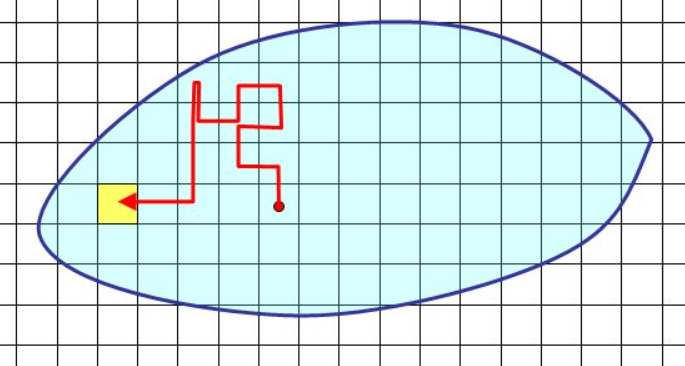
\includegraphics[width = 0.3\linewidth]{dfk-walk.png}
	\end{center} 
\end{frame}

\begin{frame}{Hit-and-run}
	The hit-and-run random walk was proved to mix in polynomial time by Lov\'{a}sz in \cite{hit-and-run-lovasz}. \pause
	\begin{defn}[Hit-and-run]
		Given $x_t$, we first draw $y$ uniformly at random from $\mathbb{S}^{n-1}$. We then draw $x_{t+1}$ uniformly at random from the set
		\[ K \cap (x_t + y\R). \]
	\end{defn}
	\pause Since the scheme is ergodic and reversible with respect to $\pi_K$, its stationary distribution is $\pi_K$. % ***** CHECK YOURSELF!
\end{frame}

\begin{frame}{Coordinate hit-and-run}
	In the simpler \emph{coordinate hit-and-run} walk (which is the subject of this presentation), we instead draw $y$ uniformly randomly from $\{e_1,\ldots,e_n\}$, the standard basis of $\Rn$. \pause \\
	In other words,
	\begin{defn}[Coordinate hit-and-run]
		For the coordinate hit-and-run (CHR) Markov scheme $\mathcal{C}$, the transition probability density from $u$ to $v$ (with respect to the $1$-dimensional Lebesgue measure) is
		\[
			\mathcal{C}_{uv} =
			\begin{cases}
				\frac{1}{n|K \cap (u + e_i\R)|}, & v \in K \cap (u+e_i\R) \text{ for some } i\in[n], \\
				0, & \text{otherwise}.
			\end{cases}
		\]
	\end{defn}
	\pause The above is also sometimes referred to as the \emph{Gibbs sampler}.
\end{frame}

\begin{frame}{Warm start}
	While we have mentioned mixing throughout in a general context, we in fact mean mixing from a `warm start'.\pause

	\begin{defn}
		A distribution $P$ is said to be \emph{$M$-warm} with respect to another distribution $Q$ if the Radon-Nikodym derivative of $P$ with respect to $Q$ is well-defined and at most $M$ at any point.
	\end{defn}

	\pause In the actual sampling process, we shall bound the mixing time assuming that we are given some distribution that is $M$-warm with respect to the stationary distribution of the chain.
\end{frame}

\begin{frame}{Conductance}
	The primary tool we use to determine how fast the Markov chains mix from a warm start is \emph{conductance}. \pause

	\begin{defn}[Conductance]
		Given a Markov scheme $P$ on $S$, the \emph{ergodic flow} $\Phi_{P,Q}$ with respect to a probability distribution $Q$ on $S$ is
		\[ \Phi_{P,Q}(A,B) = \int_A P(u,B) Q(\dif u) \]
		for measurable $A,B\subseteq S$. We also define $\Phi_{P,Q}(A) = \Phi_{P,Q}(A,S\setminus A)$. \pause \\
		For $0<s<1/2$, the \emph{$s$-conductance} of $P$ with respect to $Q$ is
		\[ \Phi_s = \inf_{A : s < Q(A) < 1/2} \frac{\Phi_{P,Q}(A)}{Q(A) - s}. \]
		The $0$-conductance is referred to as merely \emph{conductance}.
	\end{defn}
 \end{frame}

\begin{frame}{Conductance to mixing}	
	We assert the rapid mixing condition by bounding the $s$-conductance. \pause

	\begin{thm}
		If a Markov scheme $P$ has stationary distribution $Q$, and we start it with initial distribution $Q_0$ with
		\[ H_s = \sup\{|Q(A) - Q_0(A)| : \text{$A$ measurable with $Q(A) < s$}\}, \]
		\pause then
		\[ d_{\text{TV}}(Q_t,Q) \le H_s \left( 1 + \frac{1}{s} \left( 1 - \frac{\Phi_s^2}{2} \right)^t \right). \]
	\end{thm}
	\pause If $Q_0$ is $M$-warm with respect to $Q$, then $H_s \le Ms$. Setting $s = \epsilon/(2M)$, we get that
	\[ d_\text{TV}(Q_t,Q) < \epsilon \text{ if } t \ge \log(2M/\epsilon) \Phi_{s}^{-2}. \]
	\pause We give two polynomial bounds on the $s$-conductance of the CHR scheme. \pause
\end{frame}

\begin{frame}{Two bounds}
	The first bound is due to \cite{narayanan_srivastava_chr}, showing that if $B_\infty^n \subseteq K \subseteq R\cdot B_\infty^n$, then
	\[ \Phi_{\mathcal{C},s} = \Omega\left( \frac{s^2}{R^2 n^{3.5} (\log n)^3} \right). \]
	\pause

	The second is due to \cite{laddha_vempala_gibbs}, showing that if $B_2^n \subseteq K$ and $R_0^2 = \expec_{x \sim \pi_K}\norm{x - b_K}_2^2$, then
	\[ \Phi_{\mathcal{C},s} = \Omega\left( \frac{s}{R_0 n^{4.5} \log n} \right). \]
	% $R$ can be a factor of at most $n^{1/2}$ larger than $R_0$.
\end{frame}

\begin{frame}{Comparing the two bounds}
	For any body, $R$ is within a factor of $O(\sqrt{n})$ of $R_0$. Depending on the body, either of the two bounds can be better. The first bound (featuring $R$) is better for ``cube-like'' bodies, and the second bound is better for long thin ``tube-like'' bodies.
\end{frame}

\section{The first bound}
\begin{frame}{Overview of the proof}
	% The proof of this is primarily by bounding the conductance of an auxiliary Gaussian random walk from below. \pause
	\begin{defn}[Gaussian CHR]
		Given $x_t$, we draw $i$ uniformly from $[n]$ and $\kappa$ from $\mathcal{N}(0,\sigma^2)$. The next point $x_{t+1}$ is defined by
		\[
			x_{t+1} =
			\begin{cases}
				x_{t} + \kappa e_i, & (x_t + \kappa e_i) \in K, \\
				x_{t}, & \text{otherwise.}
			\end{cases}
		\]
		% The Gaussian coordinate hit-and-run (GCHR) walk $\mathcal{G}$ is defined as follows., the transition probability density from $u$ to $v$ (with respect to the $1$-dimensional Lebesgue measure) is
		% \[
		% 	\mathcal{G}(u,v) =
		% 	\begin{cases}
		% 		\frac{1}{n\sqrt{2\pi}\sigma} \exp\left( -\frac{\norm{v-u}^2}{2\sigma^2} \right), & v \ne u, v \in K \cap (u+e_i\R) \text{ for some } i\in[n], \\
		% 		0, & \text{otherwise}.
		% 	\end{cases}
		% \]
		% Note that in this case, the rejection probability 
	\end{defn}
	\pause On bounding the Radon-Nikodym derivative of $\mathcal{C}(x,\cdot)$ with respect to $\mathcal{G}(x,\cdot)$ from below, we arrive at a bound for the conductance of $\mathcal{C}$. \pause \\
	The original strategy used to prove the convergence of usual hit-and-run was to show that `close-by' points have `similar' distributions. \pause Here, we do a multistep version of the same, showing that the distributions become similar after running the walk for several steps.
\end{frame}

\begin{frame}{Some setup for the proof}
	Denote by $\mathcal{G}_v^{(\tau)}$ the probability distribution obtained on starting $\mathcal{G}$ at $v \in \Rn$ and letting it run for $\tau$ time steps. \pause \\
	
	\begin{itemize}
		\item Let $\mathcal{M}_{n,\tau}$ be the set of all $\mathbb{I} = (i_1,\ldots,i_n) \in \N^n$ with $\sum i_j = \tau$. \pause
		\item For each such $\mathbb{I}$, define $\mathcal{G}_{v,\mathbb{I}}$ as the Gaussian distribution centered at $v$ with diagonal covariance matrix $\Sigma_{\mathbb{I}}$ defined by $(\Sigma_\mathbb{I})_{jj} = \mathbb{I}_j \sigma^2$. \pause
		\item Finally, define $\lambda_{\mathbb{I}} = \binom{\tau}{\mathbb{I}} n^{-\tau}$, which is the probability of getting the multi-index $\tau$ on uniformly drawing an element of $[n]$ $\tau$ times.
	\end{itemize}
\end{frame}

\begin{frame}{Some setup for the proof (contd.)}
	Observe that if we drop the $v \in K$ condition in the definition of $\mathcal{G}$, we just get the random walk $\mathcal{H}$ defined by the mixture
	\[ \mathcal{H}_{v}^{(\tau)} = \sum_{\mathbb{I} \in \mathcal{M}_{n,\tau}} \lambda_{\mathbb{I}} \mathcal{G}_{v,\mathbb{I}}. \]
	\pause Also define
	\[ (\mathcal{H}')_{v}^{(\tau)} = \sum_{\substack{\mathbb{I} \in \mathcal{M}_{n,\tau} \\ \mathbb{I}_j \ne 0 \text{ for all }j }} \lambda_{\mathbb{I}} \mathcal{G}_{v,\mathbb{I}}. \]
\end{frame}

\begin{frame}{Showing the closeness property for $\mathcal{G}$}
	% \MyText{$\mathcal{G}_{v,\mathbb{I}} = v + \mathcal{N}(0,\sigma^2\Sigma_\mathbb{I})$}
	\MyText{$\mathcal{G}_{v,\mathbb{I}} = v + \mathcal{N}(0,\sigma^2\Sigma_\mathbb{I})$ \newline $\mathcal{H}_v^{(\tau)} = \sum_{\mathbb{I} \in \mathcal{M}_{n,\tau}} \lambda_{\mathbb{I}} \mathcal{G}_{v,\mathbb{I}}$}
	To show that close points have similar distributions, we shall first show that
	\begin{equation}
		d_{\text{TV}}(\mathcal{G}_{v}^{(\tau)} , \mathcal{H}_v^{(\tau)}) \text{ is small}
	\end{equation}
	\pause and then that for close points $u,v$,
	\begin{equation}
		d_{\text{TV}}( \mathcal{H}_u^{(\tau)} , \mathcal{H}_v^{(\tau)}) \text{ is small.}
	\end{equation}
\end{frame}

\begin{frame}{A proof of (1)}
	\MyText{$\mathcal{G}_{v,\mathbb{I}} = v + \mathcal{N}(0,\sigma^2\Sigma_\mathbb{I})$ \newline $\mathcal{H}_v^{(\tau)} = \sum_{\mathbb{I} \in \mathcal{M}_{n,\tau}} \lambda_{\mathbb{I}} \mathcal{G}_{v,\mathbb{I}}$}
	\[ d_{\text{TV}}(\mathcal{G}_{v}^{(\tau)} , \mathcal{H}_v^{(\tau)}) \text{ is small.} \]
	\pause Let $x_0 = v$. For $t \in [\tau]$, pick $i \in [n]$ uniformly randomly, $\kappa \sim \mathcal{N}(0,\sigma^2)$, and let $x_{t} = x_{t-1} + \kappa e_i$. \pause $x_\tau$ just represents a draw from $\mathcal{H}_v^{(\tau)}$. \pause \\

	Consider the event $E$ that every $x_i$ is in $K$. \pause By a standard coupling argument,
	\[ d_\text{TV}(\mathcal{G}_v^{(\tau)}, \mathcal{H}_v^{(\tau)}) \le 1 - \Pr[E]. \]
	\pause Now, set $\tau = 20 n \log n$ and suppose that $\inf_{z \in \partial K} \norm{v - z}_\infty > 100 \sigma \log n$. \pause An application of the Chernoff bound (to show that no coordinate is chosen many times) together with a Gaussian tail bound (to show that none of the coordinate changes are too large) shows that with high probability, the points remain in $K$.
\end{frame}

\begin{frame}{A proof of (2)}
	\MyText{$\mathcal{H}_v^{(\tau)} = \sum_{\mathbb{I} \in \mathcal{M}_{n,\tau}} \lambda_{\mathbb{I}} \mathcal{G}_{v,\mathbb{I}}$ \\ ${\mathcal{H}'}_v^{(\tau)} = \sum_{\substack{\mathbb{I} \in \mathcal{M}_{n,\tau} \\ \forall j, \mathbb{I}_j \ne 0}} \lambda_{\mathbb{I}} \mathcal{G}_{v,\mathbb{I}}$}
	\[ d_{\text{TV}}( \mathcal{H}_u^{(\tau)} , \mathcal{H}_v^{(\tau)}) \text{ is small.} \]
	\pause To show this, first observe that
	\[ d_{\text{TV}}(\mathcal{H}_u^{(\tau)} , (\mathcal{H}')_u^{(\tau)}) \text{ is small.} \]
	\pause Indeed, the distance between the two is at most the sum of all $\lambda_\mathbb{I}$ over all $\mathbb{I} \in \mathcal{M}_{n,\tau}$ with a zero in them, and this in turn can be made small for large $\tau$. \pause Therefore, it suffices to show that
	\[ d_{\text{TV}}( (\mathcal{H}')_u^{(\tau)} , (\mathcal{H}')_v^{(\tau)}) \text{ is small.} \]
\end{frame}

\begin{frame}{A proof of (2) (contd.)}
	For this, we use Pinsker's inequality to get that for any $\mathbb{I} \in \mathcal{M}_{n,\tau}$ with no non-zero element, \pause
	\begin{align*}
		d_{\text{TV}}( \mathcal{G}_{v,\mathbb{I}} , \mathcal{G}_{u,\mathbb{I}} ) &\le \sqrt{\frac{1}{2} D_\text{KL} (\mathcal{G}_{v,\mathbb{I}} \lVert \mathcal{G}_{u,\mathbb{I}}) } \\ 
			\uncover<3->{&= \frac{1}{2} \sqrt{ (v-u)^\top \Sigma_\mathbb{I}^{-1} (v-u) }} \\ 
			\uncover<4->{&\le \frac{1}{2\sigma} \norm{v-u}_2.}
	\end{align*}
	\pause\pause\pause Therefore,
	\[ d_{\text{TV}}( (\mathcal{H}')_u^{(\tau)} , (\mathcal{H}')_v^{(\tau)}) \le \sum_{\substack{ \mathbb{I} \in \mathcal{M}_{n,\tau} \\ \mathbb{I}_j \ne 0 \text{ for any $j$} }} \lambda_\mathbb{I} d_{\text{TV}}( \mathcal{G}_{v,\mathbb{I}} , \mathcal{G}_{u,\mathbb{I}} ) \le \frac{\norm{v-u}_2}{2\sigma}, \]
	which is small.
\end{frame}

\begin{frame}{Concluding the main proof}
	Now, consider the multistep Gaussian CHR walk $\mathcal{G}'$, performing $\tau = 20 n \log n$ steps of $\mathcal{G}$ at each step. \pause By (1) and (2), $\mathcal{G}'$ satisfies the following property. Let
	\[ K' = \{ x \in K : \inf_{z \in \partial K} \norm{x - z}_\infty > 100 \sigma \log n \}. \]
	\pause Then, for any $u,v \in K'$ with $\norm{u-v}_2 \le \textcolor{green}{\sigma}$,
	\[ d_\text{TV} (\mathcal{G}'(u,\cdot),\mathcal{G}'(v,\cdot)) \le 1 - \textcolor{blue}{\frac{1}{4}}. \]
	\pause Given that $B_\infty \subseteq K$, we may further show that $(1 - 100 \sigma \log n) K \subseteq K'$. Consequently,
	\[ \vol(K') \ge (1 - \textcolor{red}{100\sigma n \log n}) \vol(K). \]
	This is referred to as the $(\textcolor{red}{\epsilon},\textcolor{green}{\delta},\textcolor{blue}{\nu})$ property.
\end{frame}

\begin{frame}
	Now, how do we go from the $(\epsilon,\delta,\nu)$ property of $\mathcal{G}'$ to a bound on the conductance? \pause
	Let $S_1 \sqcup S_2$ be a partition of $K$ into disjoint measurable subsets. \pause Let $T_i = S_i \cap K'$ (so we may use the $(\epsilon,\delta,\nu)$ property). \pause Define
	\[ T_i' = \{ x \in T_i : \mathcal{G}'(x,S_{3-i}) < \nu/2 \}. \]
	\pause Observe that for any $x\in T_1', y \in T_2'$, $\norm{x-y}_2 > \delta$. Indeed, otherwise,
	\[ 1 - \nu \ge d_\text{TV}(\mathcal{G}'(x,\cdot), \mathcal{G}'(y,\cdot)) \ge 1 - \mathcal{G}'(x,S_2) - \mathcal{G}'(y,S_1) > 1 - \nu. \]
	\pause We now use Theorem 2.6 of \cite{vol-algo}.
	\begin{thm}
		Let $\delta > 0$ and $\norm{\cdot}_\ell$ be a norm on $\Rn$. Let $K$ be a convex body in $\Rn$ and $K_1,K_2$ be disjoint measurable subsets of $K$ such that for $u\in K_1$ and $v\in K_2$, $\norm{u-v}_\ell \ge \delta$. Further suppose that $\sup_{x,y \in K} \norm{x-y}_\ell = D$. \pause Then,
		\[ \pi_K(K \setminus (K_1 \cup K_2)) \ge \frac{2\delta}{D-\delta} \min\{\pi_K(K_1),\pi_K(K_2)\}. \] 
	\end{thm}
\end{frame}

\begin{frame}
	The previous theorem implies that
	\[ \pi_{K}(K'\setminus (T_1' \cup T_2')) \ge \frac{2\delta}{D-\delta} \min \{\pi_{K}(T_1'),\pi_{K}(T_2')\}. \]
	\pause If $\pi_K(T_1') \le \frac{1}{2} \pi_K(T_1)$, then the result immediately follows since
	\[ \Phi_{\mathcal{G}',\pi_K}(S_1,S_2) \ge \Phi_{\mathcal{G}',\pi_K}(T_1\setminus T_1',S_2) \ge \frac{\nu}{4} (\pi_K(S_1) - \epsilon). \]
	\pause Therefore, assume that $\pi_K(T_i') > \frac{1}{2} \pi_K(T_i)$. \pause We now have
	\begin{align*}
		\Phi_{\mathcal{G}', \pi_K}(S_1,S_2) &\ge \frac{1}{2} ( \Phi_{\mathcal{G}', \pi_K}(T_1 \setminus T_1',S_2) + \Phi_{\mathcal{G}', \pi_K}(S_1,T_2\setminus T_2') ) \\
			\uncover<5->{&\ge \frac{\nu}{4} ( \pi_K(T_1 \setminus T_1') + \pi_K(T_2 \setminus T_2') )} \\
			\uncover<6->{&= \frac{\nu}{4} ( \pi_K(K' \setminus (T_1' \cup T_2')) )} \\
			\uncover<7->{&\ge \frac{\nu\delta}{2(D-\delta)} \min\{\pi_K(T_1'), \pi_K(T_2')\}} \\
			\uncover<8->{&\ge \frac{\nu\delta}{4(D-\delta)} (\min\{\pi_K(S_1),\pi_K(S_2)\} - \epsilon).} 
	\end{align*}
	\pause\pause\pause\pause\pause This gives a bound on the $\epsilon$-conductance of $\mathcal{G}'$!
\end{frame}

\begin{frame}{Going from $\mathcal{G}'$ to $\mathcal{G}$}
	Now, we must arrive at a bound on the conductance of $\mathcal{G}$. Fix some measurable $S \subseteq K$. \pause Let $x_0,x_1,\ldots,x_\tau$ be a walk according to the scheme $\mathcal{G}$, where $x_0$ is sampled from $\pi_K$. \pause Let $E$ denote the event that $x_0 \in S$ and $x_\tau \in K \setminus S$, and $E_i$ the event that $x_i \in S$ and $x_{i+1} \in K \setminus S$. \pause Clearly, $\Pr[E] \le \sum_{i} \Pr[E_i]$. \pause\\
	Since each $x_i$ is sampled from $\pi_K$ (the stationary distribution of $\mathcal{G}$ is $\pi_K$), $\Pr[E_i] = \Phi_{\mathcal{G},\pi_K}(S,K\setminus S)$. \pause Further, $\Pr[E] = \Phi_{\mathcal{G}',\pi_K}(S,K\setminus S)$. \pause It follows that
	\[ \Phi_{\mathcal{G},\pi_K}(S,K\setminus S) \ge \frac{1}{\tau} \Phi_{\mathcal{G}',\pi_K}(S,K\setminus S). \]
\end{frame}

\begin{frame}{Completing the proof}
	Finally, since the Radon-Nikodym derivative of $\mathcal{C}(x,\cdot)$ with respect to $\mathcal{G}(x,\cdot)$ at $y \neq x$ is bounded below by $\sqrt{2\pi}\sigma/2R$ at any point, \pause
	\begin{align*}
		\Phi_{\mathcal{C},\pi_K}(S,K\setminus S) &\ge \frac{\sqrt{2\pi}\sigma}{2R\tau} \Phi_{\mathcal{G}',\pi_K}(S,K\setminus S) \\
			\uncover<3->{&\ge \frac{\sqrt{2\pi}\sigma}{2R\tau} \cdot \frac{\nu\delta}{4(D-\delta)} (\min\{\pi_K(S),\pi_K(K\setminus S)\} - \epsilon) }
	\end{align*}
	\pause\pause Substituting $\tau = 20 n\log n$, $\nu = 1/4$, $\delta = \sigma$, $\epsilon = s$, $\sigma = 32s/(n\log n)$ and using the fact that $D \le R\sqrt{n}$, \pause we get
	\[ \Phi_{\mathcal{C},\pi_K}(S,K\setminus S) \ge \frac{cs^2}{R^2n^{3.5}(\log n)^3} (\min\{\pi_K(S),\pi_K(K\setminus S)\} - \epsilon), \]
	completing the proof.
\end{frame}

\section{The second bound}
\begin{frame}{Overview of the proof}
	In this proof, we reduce the problem of bounded conductance to that of an isoperimetric problem on `axis-disjoint' subsets. \pause
	\begin{defn}
		Sets $S_1,S_2 \subseteq \Rn$ are said to be \emph{axis-disjoint} if for any $i \in [n]$, $(S_1 + e_i\R) \cap S_2 = \emptyset$.
	\end{defn}
	\pause Similar to how in the earlier proof we used the $(\epsilon,\delta,\nu)$ property to arrive at an isoperimetric inequality, here we use the following theorem to get the same.
\end{frame}

\begin{frame}{The main result}
	\begin{thm}
		\label{mainthm-2}
		Let $K$ be a convex body satisfying $B_2^n \subseteq K$ and let $R_0^2 = \expec_{x \sim \pi_K}\norm{x - b_K}_2^2$, where $b_K$ is the centroid of $K$. Let $S_1, S_2 \subseteq K$ be axis-disjoint. Then, there exists a universal constant $c$ such that for any $\epsilon>0$,
		\[ \pi_K(K \setminus (S_1 \cup S_2)) \ge \frac{c\epsilon}{R_0 n^{3.5} \log n} ( \min\{\pi_K(S_1),\pi_K(S_2)\} - \epsilon ). \]
	\end{thm}
	\pause We denote $K\setminus (S_1 \cup S_2)$ as $S_3$. \\
	\pause To prove this, we consider a grid of cubes, proving an isoperimetric inequality on each of them separately, then combining these together to give a global isoperimetric inequality.
\end{frame}

\begin{frame}{The final part of the proof}
	Before proving Theorem \ref{mainthm-2}, let us show how a bound on the conductance follows from it. \pause Suppose $S_1 \sqcup S_2$ is a partition of $K$ into disjoint measurable subsets. \pause Set
	\[ S_i' = \left\{ x \in S_i : \mathcal{C}(x,S_{3-i}) < \frac{1}{2n} \right\}. \]
	\pause We claim that $S_1'$ and $S_2'$ are axis-disjoint. \pause Otherwise, let $\ell$ be an axis-parallel line intersecting both of them. If $x_i \in \ell \cap S_i'$,
	\[ \frac{1}{2n} > \mathcal{C}(x_i,S_{3-i}) \ge \frac{1}{n} \frac{|\ell \cap S_i|}{|\ell \cap K|}. \]
	\pause However, this gives that $|\ell\cap K| > |\ell \cap S_1| + |\ell \cap S_2|$, which is clearly incorrect since the two are equal. \pause \\
	The remainder of the proof follows near-identically to the final part of the proof of the first bound, except that instead of the $(\epsilon,\delta,\nu)$ property to bound conductance, we use the given theorem regarding axis-disjoint sets.
\end{frame}

\begin{frame}{Isoperimetry on a cube}
	The following isoperimetric inequality is not too hard to prove and we use it extensively.
	\begin{lem}
		% \label{cube-isoperimetry}
		Let $C$ be an axis-aligned cube in $\Rn$. For any axis-disjoint $S_1,S_2 \subseteq C$,
		\[ \pi_C(C \setminus (S_1 \cup S_2)) \ge \frac{1}{4n\log n} \min\{\pi_C(S_1), \pi_C(S_2)\}. \]
	\end{lem}

	\pause Since we have by definition that
	\[ \pi_C(C \setminus (S_1 \cup S_2)) \ge 1 - \pi_C(S_1) - \pi_C(S_2), \]
	\pause we also have that if $\pi_C(S_1) \le (2/3)$,
	\begin{equation}
		\label{eqn 3}
		\pi_C(C \setminus (S_1 \cup S_2)) \ge \frac{1}{16n\log n} \pi_C(S_1).
	\end{equation}
\end{frame}

\begin{frame}{The lattice}
	We now move on to the proof of the result. Let $S_1,S_2$ be axis-disjoint subsets of $K$. Similar to the first proof, set $K' = (1 - \epsilon/20n)K$, and let $S_i' = S_i \cap K'$. Suppose $\vol(S_1') \le \vol(S_2')$. \pause \\ 
	Consider the lattice $\delta\Z^n$, where $\delta = \epsilon/80n\sqrt{n}$. This value of $\delta$ is chosen to ensure that any of the cubes that intersect $S_i'$ are contained completely within $K$. \pause \\
	Define $\mathcal{C}$ to be the set of hypercubes in the lattice that intersect $S_1$, $\mathcal{C}_1$ as the set of cubes in $\mathcal{C}$ where $S_1$ takes up at most $2/3$ the volume of the cube, and $\mathcal{C}_2$ as $\mathcal{C} \setminus \mathcal{C}_1$.
\end{frame}

\begin{frame}{The case where $\mathcal{C}_1$ has many cubes}
	If there is a significant number of cubes in $\mathcal{C}_1$, that is, $\vol(\mathcal{C}_1 \cap S_1) \ge \vol(S_1)/2$, then we can use the previous isoperimetry on each of the cubes to arrive at an overall isoperimetric inequality. \pause That is, we have
	\begin{align*}
		\pi_K(S_3) &\ge \frac{1}{16n\log n} \sum_{\substack{c \in \mathcal{C}_1 \\ c \cap K' \ne \emptyset}} \pi_K(c \cap S_1) \\
			\uncover<3->{&\ge \frac{1}{16n\log n} \left(\pi_K(\mathcal{C}_1 \cap S_1) - \frac{\epsilon}{2}\right)} \\
			\uncover<4->{&\ge \frac{1}{32n\log n} \left( \pi_K(S_1) - \epsilon \right).}
	\end{align*}
\end{frame}

\begin{frame}{The non-trivial part}
	Therefore, suppose that $\vol(\mathcal{C}_2 \cap S_1) \ge \vol(S_1)/2$.\\ 
	\pause The idea is as follows. We first show that the cubes adjacent to $\partial \mathcal{C}_2$ not in $\mathcal{C}_2$ have a significant amount of $S_3$\pause, then use a known isoperimetric inequality to compare the volume of $\mathcal{C}_2$ to that of $\partial \mathcal{C}_2$.\pause \\
	Combining these two inequalities compares the volume of $\mathcal{C}_2$ (and thus $S_1$) to that of $S_3$, which is exactly what we desire.\pause\\
	Set $\mathcal{C}_2'$ to be the set of cubes in $\mathcal{C}_2$ that intersect $K'$.
\end{frame}

\begin{frame}{The isoperimetric inequality (1)}
	First, let us show the second part in the overview described on the previous slide. \pause In \cite{KLS}, Kannan, Lov\'{a}sz, and Simonovits show that for any convex body $K$ and measurable $S \subseteq K$,
	\begin{equation}
		\label{eqn-kls}
		\vol(\partial_{K}(S)) \ge \frac{\log 2}{R_0} \min\{ \vol(S) , \vol(K\setminus S) \},
	\end{equation}
	where $\partial_K(S)$ is the boundary of $S$ relative to $K$. \\
	\pause In particular, since we have
	% \[ \vol(\mathcal{C}_2' \cap S_1) \le \vol(\mathcal{C}_2') \le \frac{3}{2} \vol(S_1 \cap K') \le \frac{3}{4} \vol(K'), \]
	\[ \vol(\mathcal{C}_2') \le \frac{3}{2} \vol(S_1 \cap K') \le \frac{3}{4} \vol(K'), \]
	it follows that
\end{frame}

\begin{frame}{The isoperimetric inequality (2)}
	\begin{align*}
		\vol(\partial_{K'}(\mathcal{C}_2')) &\ge \frac{\log 2}{R_0} \min\{ \vol(\mathcal{C}_2') , \vol(K' \setminus \mathcal{C}_2') \} \\
			\uncover<2->{&\ge \frac{\log 2}{R_0} \min\left\{ \vol(\mathcal{C}_2') , \frac{1}{4} \vol(K') \right\}} \\
			\uncover<3->{&\ge \frac{\log 2}{R_0} \min\left\{ \vol(\mathcal{C}_2 \cap K') , \frac{1}{4} \vol(\mathcal{C}_2 \cap K') \right\}} \\
			\uncover<4->{&= \frac{\log 2}{4R_0} \vol(\mathcal{C}_2 \cap K')} \\
			\uncover<5->{&\ge \frac{\log 2}{4R_0} \left(\frac{1}{2}\vol(S_1) - \frac{\epsilon}{2} \vol(K)\right)} \\
			\uncover<6->{&= \frac{\log 2}{8R_0} \left( \vol(S_1) - \epsilon \vol(K) \right).}
	\end{align*}
	\pause\pause\pause\pause\pause\pause If we manage to compare $\vol(S_3)$ and $\vol(\partial_{K'}(\mathcal{C}_2'))$, we are done.
\end{frame}

\begin{frame}{Comparing $\vol(S_3)$ and $\vol(\partial_{K'}(\mathcal{C}_2'))$ (1)}
	Since $\mathcal{C}_2$ is a set of cubes, its boundary consists of facets. \pause Let $f$ be one such facet, $c_2$ be the cube adjacent to it that is in $\mathcal{C}_2$, and $c_1$ be the other cube adjacent to it.\\
	\pause Since $\vol(c_2 \cap S_1) \ge (2/3) \vol(c_2)$, at least $2/3$ of $c_1$ is reachable from $S_1$, and is thus not in $S_2$.\\
	\pause We then have two cases:
	\begin{enumerate}
		\item \pause If $\vol(c_1 \cap S_1) \le \vol(c_1)/3$, at least $1/3$ of the $2/3$ fraction earlier (that is not in $S_2$) is not in $S_1$ either, and is thus in $S_3$.
		\item \pause If $\vol(c_1)/3 \le \vol(c_1 \cap S_1) \le 2\vol(c_1)/3$, we can use (\ref{eqn 3}) to conclude that
		\[ \vol(c_1 \cap S_3) \ge \frac{1}{16 n \log n} \vol(c_1 \cap S_1) \ge \frac{1}{48n\log n} \vol(c_1). \]
	\end{enumerate}
\end{frame}

\begin{frame}{Comparing $\vol(S_3)$ and $\vol(\partial_{K'}(\mathcal{C}_2))$ (2)}
	The above says that each cube adjacent to a facet of $\partial_K(\mathcal{C}_2)$ that is not in $\mathcal{C}_2$ must have at least a $1/(48 n \log n)$ fraction of $S_3$. \pause Since each such cube is adjacent to at most $2n$ facets, each facet to contributes to a $S_3$ volume at least
	\[ \frac{1}{96 n^2 \log n} \delta^n. \]
	\pause That is,
	\begin{align*}
		\vol(S_3) &\ge \sum_{f \in \partial_{K'}(\mathcal{C}_2')} \frac{1}{96n^2 \log n} \delta^n \\
			\uncover<4->{&= \frac{\delta}{96n^2 \log n} \sum_{f \in \partial_{K'}(\mathcal{C}_2')} \delta^{n-1}} \\
			\uncover<5->{&= \frac{\delta}{96n^2 \log n} \vol(\partial_{K'}(\mathcal{C}_2')).}
	\end{align*}
\end{frame}

\begin{frame}{Putting the two pieces together}
	Combining the two equations,
	\begin{align*}
		\vol(S_3) &\ge \frac{\delta}{96n^2 \log n} \vol(\partial_{K'}(\mathcal{C}_2')) \\
			\uncover<2->{&\ge \frac{\delta}{96n^2 \log n} \cdot \frac{\log 2}{8R_0} \left( \vol(S_1) - \epsilon \vol(K) \right)} \\
			\uncover<3->{&= \frac{c\delta}{R_0 n^2 \log n} \left( \vol(S_1) - \epsilon \vol(K) \right)} \\
			\uncover<4->{&= \frac{c'\epsilon}{R_0 n^{3.5} \log n} \left( \vol(S_1) - \epsilon \vol(K) \right),}
	\end{align*}
	\pause\pause\pause completing the proof.
\end{frame}

\begin{frame}{}
  \centering \Huge
  \emph{Thank you!}
\end{frame}


\begin{frame}[allowframebreaks,t]{References}
	\bibliographystyle{alpha}
	\small\bibliography{references}
\end{frame}

\end{document}